%%%%%%%%%%%%%%%%%%%%%%%%%%%%%%%%%%%%%%%%%
% Masters Thesis 
% LaTeX Template
%
% This template is based on a template by:
% Steve Gunn (http://users.ecs.soton.ac.uk/srg/softwaretools/document/templates/)
% Sunil Patel (http://www.sunilpatel.co.uk/thesis-template/)
%
% Template license:
% CC BY-NC-SA 3.0 (http://creativecommons.org/licenses/by-nc-sa/3.0/)
%
%%%%%%%%%%%%%%%%%%%%%%%%%%%%%%%%%%%%%%%%%

%----------------------------------------------------------------------------------------
%	PACKAGES AND OTHER DOCUMENT CONFIGURATIONS
%----------------------------------------------------------------------------------------

\documentclass[
11pt, % The default document font size, options: 10pt, 11pt, 12pt
%oneside, % One-sided layout avoids blank pages between chapters
english, % ngerman for German
singlespacing, % Single line spacing, alternatives: onehalfspacing or doublespacing
%draft, % Uncomment to enable draft mode (no pictures, no links, overfull hboxes indicated)
%nolistspacing, % If the document is onehalfspacing or doublespacing, uncomment this to set spacing in lists to single
%liststotoc, % Uncomment to add the list of figures/tables/etc to the table of contents
%toctotoc, % Uncomment to add the main table of contents to the table of contents
%parskip, % Uncomment to add space between paragraphs
%nohyperref, % Uncomment to not load the hyperref package
headsepline, % Uncomment to get a line under the header
%chapterinoneline, % Uncomment to place the chapter title next to the number on one line
%consistentlayout, % Uncomment to change the layout of the declaration, abstract and acknowledgements pages to match the default layout
]{MastersDoctoralThesis} % The class file specifying the document structure

\usepackage[utf8]{inputenc} % Required for inputting international characters
\usepackage[T1]{fontenc} % Output font encoding for international characters

\usepackage{mathpazo} % Use the Palatino font by default

\usepackage[backend=biber,style=numeric,sorting=none,natbib=true]{biblatex} % Use numbered citations and bibliography entries

\addbibresource{example.bib} % The filename of the bibliography

\usepackage[autostyle=true]{csquotes} % Required to generate language-dependent quotes in the bibliography
\usepackage{tabularx} % Flexible-width tables

\usepackage[htt]{hyphenat}
\usepackage{xurl}

%----------------------------------------------------------------------------------------
%	MARGIN SETTINGS
%----------------------------------------------------------------------------------------

\geometry{
    paper=a4paper,
    inner=2.5cm,
    outer=3.8cm,
    bindingoffset=.5cm,
    top=1.5cm,
    bottom=1.5cm,
    %showframe,
}

%----------------------------------------------------------------------------------------
%	THESIS INFORMATION
%----------------------------------------------------------------------------------------

\thesistitle{Causal Machine Learning for Markdown Price Optimization in Retail} % Thesis title
\supervisor{Oriol Pujol Vila\\Daniel Guti\'errez Meyer} % Academic and external supervisors
\examiner{} % Optional
\degree{MSc in Fundamentals of Data Science} % Degree name
\author{Joel Sanfeliu Ichihashi} % Author name
\addresses{} % Your address, this is not currently used anywhere in the template, print it elsewhere with \addressname

\subject{Data Science} % Subject area
\keywords{causal inference, double machine learning, price elasticity, markdown optimization, retail analytics} % PDF keywords
\university{\href{http://www.ub.edu}{Universitat de Barcelona}} % Your university's name and URL, this is used in the title page and abstract, print it elsewhere with \univname
\department{} % Optional department name
\group{Mango} % Collaborating company
\faculty{\href{http://mat.ub.edu}{Facultat de Matemàtiques i Informàtica}} % Your faculty's name and URL, this is used in the title page and abstract, print it elsewhere with \facname

\AtBeginDocument{
\hypersetup{pdftitle=\ttitle} % Set the PDF's title to your title
\hypersetup{pdfauthor=\authorname} % Set the PDF's author to your name
\hypersetup{pdfkeywords=\keywordnames} % Set the PDF's keywords to your keywords
}

\makeatletter
\renewcommand{\@makechapterhead}[1]{%
	\abovechapterskip
	{\parindent \z@ \chapteralign \normalfont
		\interlinepenalty\@M%
		\chapterfont #1\par\nobreak
		\chapterbelowskip
	}
	\thispagestyle{\chapter@p@gestyle}
}
\makeatother

\renewcommand{\chaptermarkformat}{}
\renewcommand{\sectionmarkformat}{}

\begin{document}

\frontmatter % Use roman page numbering style (i, ii, iii, iv...) for the pre-content pages

\pagestyle{plain} % Default to the plain heading style until the thesis style is called for the body content

%----------------------------------------------------------------------------------------
%	TITLE PAGE
%----------------------------------------------------------------------------------------

\begin{titlepage}
\begin{center}

\vspace*{.06\textheight}
{\scshape\LARGE \univname\par}\vspace{1.5cm} % University name
\textsc{\Large Fundamental Principles of Data Science Master's Thesis}\\[0.5cm] % Thesis type

\HRule \\[0.4cm] % Horizontal line
{\huge \bfseries \ttitle\par}\vspace{0.4cm} % Thesis title
\HRule \\[1.5cm] % Horizontal line
 
\begin{minipage}[t]{0.4\textwidth}
\begin{flushleft} \large
\emph{Author:}\\
\authorname % Author name - remove the \href bracket to remove the link
\end{flushleft}
\end{minipage}
\begin{minipage}[t]{0.4\textwidth}
\begin{flushright} \large
\emph{Supervisors:} \\
\supname % Supervisor name - remove the \href bracket to remove the link  
\end{flushright}
\end{minipage}\\[3cm]
 
\vfill

\large \textit{A thesis submitted in partial fulfillment of the requirements\\ for the degree of \degreename}\\[0.3cm] % University requirement text
\textit{in the}\\[0.4cm]
\facname\\[0.8cm] % Faculty name
\textit{In collaboration with Mango}\\[1.2cm]
 
\vfill

{\large \today}\\[4cm] % Date
%\includegraphics{Logo} % University/department logo - uncomment to place it
 
\vfill
\end{center}
\end{titlepage}


%----------------------------------------------------------------------------------------
%	ABSTRACT PAGE
%----------------------------------------------------------------------------------------

\begin{abstract}
\addchaptertocentry{\abstractname} % Add the abstract to the table of contents
This thesis develops a causal machine learning framework for markdown price optimization in fashion retail. The objective is to improve the elasticity curves used by the existing markdown optimizer, which under a purely predictive approach often recommends the minimum allowed discount instead of identifying a balanced markdown level. This is problematic because markdown pricing should balance the increase in demand from deeper discounts against the loss in unit price.

Using historical sales and pricing data from Mango, the study applies Double Machine Learning to control for pre-pricing factors such as stock, previous sales, product characteristics, and calendar timing. A Causal Forest is then used to estimate heterogeneous price effects, allowing the demand response to vary across products and moments of the sales campaign.

The final model is selected after comparing alternative causal specifications and is chosen for its ability to generate smoother and more economically reasonable markdown curves. The results show that the causal approach maintains predictive performance while improving the quality of the simulated curves used by the optimizer. The proposed framework therefore improves the curve-generation step while remaining compatible with the existing optimization pipeline.

\end{abstract}

%----------------------------------------------------------------------------------------
%	ACKNOWLEDGEMENTS
%----------------------------------------------------------------------------------------

\begin{acknowledgements}
\addchaptertocentry{\acknowledgementname} % Add the acknowledgements to the table of contents
I would like to thank Mango for giving me the opportunity to work on this project and to learn from a real business problem with direct practical relevance. I am especially grateful to the pricing team at Mango, who welcomed me, helped me understand the markdown process, and made this experience both valuable and enjoyable. They are an excellent team, and their support made a real difference throughout the thesis.

I would like to give special thanks to my internal supervisor at Mango, Daniel Guti\'errez Meyer. His guidance was especially helpful for noticing important details that I was missing and understanding difficult concepts. I also really appreciated our research discussions, from deciding which experiments to run to interpreting the results and thinking about their practical implications.

I am also very grateful to my university supervisor, Oriol Pujol Vila, for his feedback and encouragement. His advice helped me approach the problem in a more structured way, improve the work as it developed, and gain confidence that the direction of the thesis was the right one.

\vspace{1.5cm}
\begingroup
\raggedright
\noindent\textbf{Use of Generative AI Declaration} \\
\vspace{0.3cm}
\small
In compliance with the guidelines of the Universitat de Barcelona, I used Large Language Models (LLMs) as a supportive tool during this project. They acted as an interactive assistant to review Causal Machine Learning theory, explore model frameworks (Double Machine Learning and Causal Forests), assist with Python coding and \LaTeX\ syntax, and refine the grammatical clarity and academic tone of my original drafts. All experimental designs, modeling choices, empirical analyses, and final conclusions were executed by me.
\endgroup

\end{acknowledgements}

\tableofcontents




%----------------------------------------------------------------------------------------
%	THESIS CONTENT - CHAPTERS
%----------------------------------------------------------------------------------------

\mainmatter % Begin numeric (1,2,3...) page numbering

\pagestyle{thesis} % Return the page headers back to the "thesis" style

% Include the chapters of the thesis as separate files from the Chapters folder
% Uncomment the lines as you write the chapters

\chapter{Introduction}

\label{Chapter1}

\section{Business Context and Motivation}

Mango is a global fashion retailer present in over 120 countries. During sales periods, products go through progressive markdowns over six consecutive weeks, and the quality of these discount decisions directly affects both revenue and end-of-season stock liquidation.

Each product reference receives a weekly discount that can stay constant or increase over time, but not decrease. The decision is also constrained by predefined minimum and maximum discount limits and other business rules. This creates the central trade-off of markdown pricing: deeper discounts increase demand but reduce the unit price.

The existing pipeline combines a LightGBM demand model \cite{ke2017lightgbm} with an optimization module. This thesis does not redesign the optimizer; it focuses on improving the elasticity curves used as its input. In the current predictive approach, simulated curves tend to recommend minimum discounts rather than finding a balanced middle ground.

\section{Problem Statement and Hypothesis}

In practice, historical discounts were far from random. Business teams naturally set prices by looking at stock, previous sales, product characteristics, and expected demand. Products with weak momentum or high remaining stock are more likely to receive deeper discounts, while strong-selling products usually receive smaller markdowns. Therefore, the observed relationship between discounts and sales does not necessarily represent the causal effect of changing price.

Crucially, a model can be highly accurate at predicting historical sales and still produce unrealistic price-response curves when alternative discounts are simulated. The hypothesis of this thesis is that a causal machine learning approach can generate more reasonable markdown elasticity curves than the predictive baseline, while remaining compatible with the current optimization pipeline.

\section{Objectives}
\label{sec:objectives}

The objective of this thesis is to replace the current predictive elasticity generator with a causal alternative. The proposed model should produce plausible price-response curves with interior optima rather than frequently getting stuck at the minimum allowed discount, while preserving forecast quality as a secondary diagnostic. It should also estimate heterogeneous effects at reference-week level and provide curves that can be used by the existing optimizer without changing its business constraints or interface.
\chapter{Data Understanding}

\label{Chapter2}

\section{Original Dataset Description}

The data comes from Mango's internal demand forecasting system. The original dataset is at reference-day level: each row corresponds to a sales prediction for a specific article and day, generated from a previous prediction snapshot. The empirical analysis is restricted to the Spain market and the Woman division, which keeps the setting homogeneous while preserving the markdown-pricing structure of the original pipeline.

The available variables can be grouped into six categories, summarized in Table~\ref{tab:original-dataset-groups}. The dataset contains identification variables, product information, calendar variables, in-season commercial KPIs, price variables, and the sales target. Most of these variables are not of interest by themselves, but they describe the commercial context available before the markdown decision is made. This context is important because it may influence both the discount assigned by the business and the future sales of the product.

Throughout the thesis, original price refers to \mbox{\texttt{full\_price}}, discounted price refers to \mbox{\texttt{actual\_price}}, discount refers to \mbox{\texttt{discount}}, and units sold refers to \mbox{\texttt{y}}.

\begin{table}[h]
\centering
\small
\begin{tabularx}{\textwidth}{p{3.0cm} X}
\textbf{Group} & \textbf{Description} \\
\hline
Identification variables & Product reference, season, market, and prediction-snapshot identifiers used to anchor each observation in time. \\
Product variables & Product family, original season price, and other reference-level characteristics. \\
Calendar variables & Position of the observation within the sales period, including sales week and timing variables. \\
In-season KPIs & Pre-pricing sales and stock indicators, such as accumulated sales, average sales, stock level, coverage, and season performance. \\
Price variables & Original price (\mbox{\texttt{full\_price}}), discounted price (\mbox{\texttt{actual\_price}}), and discount (\mbox{\texttt{discount}}). \\
Target variable & units sold (\texttt{y}), later aggregated to weekly demand for modelling. \\
\end{tabularx}
\caption{Variable groups in the original dataset.}
\label{tab:original-dataset-groups}
\end{table}

\section{From Daily to Weekly}

The original data contains several daily rows for each product reference, generated from different prediction origins. However, markdown decisions are taken at weekly level. For this reason, the dataset is transformed so that the modelling unit matches the business decision unit.

For each sales week, only the snapshot taken three weeks before the start of the week is kept. This anchor is used because it represents the information available before the discount is decided. Keeping this timing is important for the causal setup: stock, accumulated sales, and other context variables must be measured before the discount decision is made, not after it. Daily sales are then aggregated into \mbox{\texttt{y\_week = sum(y)}}, while the context variables are taken from the three-week-prior snapshot.

The final dataset contains one row per reference $\times$ season $\times$ sales week, with sale weeks ranging from 1 to 6. The train-test split is season-based: three seasons are used for training and one season is held out for testing.

\begin{table}[h]
\centering
\small
\begin{tabular}{lrrrrrr}
\textbf{Split} & \textbf{Rows} & \textbf{Seasons} & \textbf{References} & \textbf{Sale weeks} & \textbf{Mean units} & \textbf{Median units} \\
\hline
Train & 33,691 & 3 & 5,790 & 1--6 & 178.4 & 53 \\
Test & 12,136 & 1 & 2,079 & 1--6 & 158.0 & 48 \\
\end{tabular}
\caption{Weekly modelling sample used in the empirical analysis.}
\label{tab:weekly-sample-summary}
\end{table}

The elasticity simulation uses the operational discount grid from 20\% to 70\%, which is the relevant support for the optimizer. Some raw historical observations can fall outside this interval, but the simulation is restricted to the range used in the curve diagnostics and in the optimization step.

For modelling, the raw weekly target is normalized by a season-level demand index, computed as the median average daily gross sales within the season. The resulting variable, \mbox{\texttt{y\_week\_per\_season\_trend}}, reduces differences in overall demand scale across seasons. This normalized variable is the final target variable used in the causal specification.

\section{Variables Used for Modelling}
\label{sec:variables-modelling}

The final modelling dataset contains three types of variables. The target variable is the season-normalized version of units sold, \mbox{\texttt{y\_week\_per\_season\_trend}}. The main price variable is discounted price (\mbox{\texttt{actual\_price}}). The discount (\mbox{\texttt{discount}}) is also available and satisfies
\[
\mbox{\texttt{actual\_price}} = \mbox{\texttt{full\_price}} \times (1 - \mbox{\texttt{discount}}),
\]
where \mbox{\texttt{full\_price}} is the original price.

The remaining variables are pre-pricing covariates describing the commercial context of each reference-week. They include calendar position, product family, original price, stock, coverage, accumulated sales performance, pre-sales indicators, and material composition when available. These variables are used as controls because they are observed before the weekly discount and summarize the information that may confound the relationship between price and demand. In the next chapter, this structure is interpreted from a causal perspective.

\chapter{Theoretical Framework}

\label{Chapter3}

\section{Causal Setup and the Markdown DAG}
\label{sec:causal-setup-dag}

The pricing question is causal rather than purely predictive: what would happen to weekly sales if the same reference-week were assigned a different price? Historical associations cannot answer this directly because markdowns are not randomized. Products with weak momentum or high remaining stock are more likely to receive deeper discounts, so discount and sales can be negatively associated even when the causal effect of a discount on demand is positive.

In causal inference, this setup can be described through three main concepts: treatment, outcome, and confounders. The treatment is the decision or variable whose effect is being studied, the outcome is the result being measured, and confounders are background variables that influence both the treatment and the outcome. Without controlling for these confounders, the estimated relationship between price and sales may confuse the true customer demand response with background factors such as product timing, stock pressure, or prior sales momentum.

A Directed Acyclic Graph (DAG) makes this structure explicit \cite{pearl2009causality}. Using the variables introduced in Chapter~\ref{Chapter2}, the treatment is discounted price, the selling price after markdown, and the outcome is weekly units sold. The confounders are the pre-pricing context variables described in Section~\ref{sec:variables-modelling}. These variables capture calendar timing, product characteristics, original price, stock pressure, sales momentum, and material composition before the markdown decision is made.

\begin{figure}[ht]
    \centering
    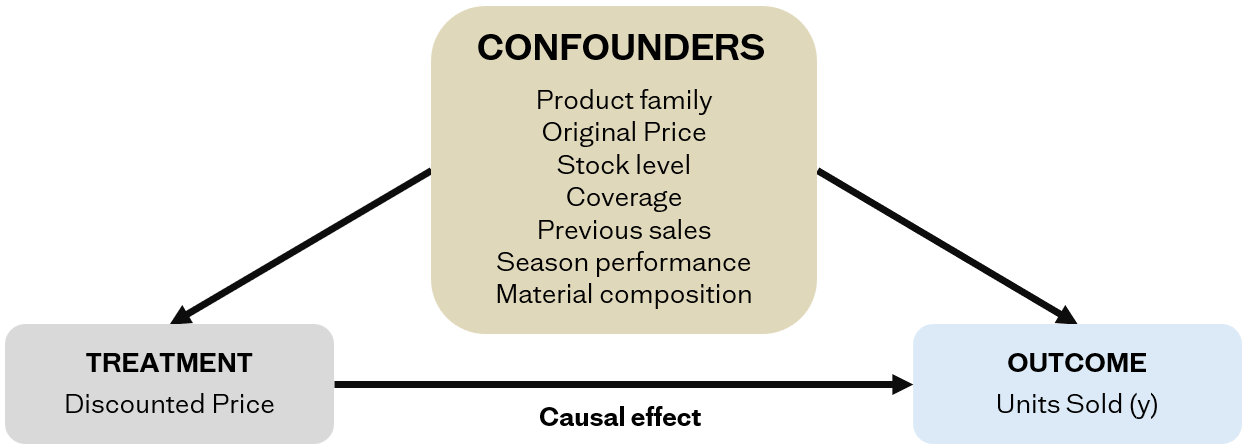
\includegraphics[width=0.95\textwidth]{Figures/dag.png}
    \caption{Simplified DAG for the markdown pricing causal setup.}
    \label{fig:markdown-dag}
\end{figure}

Figure~\ref{fig:markdown-dag} summarizes the main identifying assumption: the confounders can affect both the assigned price and future sales, while the causal effect of interest runs from the price decision to weekly demand. No variables observed after the price is set are included, as this would distort the estimated causal effect. This clear separation motivates the use of the Double Machine Learning (DML) method explained in the next sections.


\section{Potential Outcomes and Double Machine Learning}
\label{sec:potential-outcomes-dml}

The potential outcomes framework defines $Y(t)$ as the weekly sales that would be observed if a reference-week were assigned treatment level $t$ \cite{rubin1974causal,imbens2015causal}. Only one potential outcome is observed for each reference-week, so identification requires unconfoundedness: conditional on $X$, the remaining variation in price is treated as if it were random for estimating demand response \cite{angrist2009mostlyharmless}. In the continuous-treatment specification used in this thesis, the causal effect is represented by a marginal parameter, $\theta$, which approximates the expected change in demand caused by a one-unit change in price. Double Machine Learning (DML) implements this adjustment with flexible nuisance models while targeting this causal parameter \cite{chernozhukov2018dml}. The partially linear model is

\begin{equation}
Y = \theta T + g(X) + \varepsilon,
\label{eq:plr-model}
\end{equation}

where $Y$ is sales, $T$ is price, $g(X)$ captures the structural non-linear effect of context, and $\theta$ is the average marginal causal effect.

To isolate $\theta$ without relying on strict parametric assumptions, DML separates the estimation of the background context from the causal relationship itself. Let $l(X)=\mathbb{E}[Y\mid X]$ represent the expected demand given the commercial context, and let $m(X)=\mathbb{E}[T\mid X]$ represent the expected price dictated by historical pricing rules. These nuisance functions are used to remove the explainable components from both variables. Specifically, the DML algorithm proceeds in three steps for each observation $i$:

\begin{enumerate}
    \item \textbf{Residualize the outcome}: Estimate the expected demand, $\hat{l}(X_i)$, and compute the demand residual:
    \begin{equation}
    \tilde{Y}_i = Y_i - \hat{l}(X_i).
    \end{equation}
    \item \textbf{Residualize the treatment}: Estimate the expected price, $\hat{m}(X_i)$, and compute the price residual:
    \begin{equation}
    \tilde{T}_i = T_i - \hat{m}(X_i).
    \end{equation}
    \item \textbf{Estimate the causal effect}: Regress the demand residuals $\tilde{Y}_i$ on the price residuals $\tilde{T}_i$ to obtain the causal estimate $\hat{\theta}$.
\end{enumerate}

The intuition behind this process is to ask what remains after the usual business context has been stripped away. In the first step, LightGBM predicts demand using only the background variables $X$. Subtracting this prediction gives the demand residual, $\tilde{Y}_i$, which represents the portion of sales not explained by stock, timing, product characteristics, or past performance. In the second step, the same logic is applied to price. The price residual, $\tilde{T}_i$, captures the portion of the assigned price that deviates from the historical markdown policy. Regressing $\tilde{Y}_i$ on $\tilde{T}_i$ then measures how these two unexplained components move together, isolating the price effect from the confounding influence of the pre-pricing context.

In this thesis, the nuisance models are estimated with LightGBM and cross-fitting is done by season to prevent temporal leakage. Crucially, the resulting orthogonal score structure of DML makes the final estimate less sensitive to first-order approximation errors in the machine learning nuisance models, which permits flexible machine learning in the first two stages while still targeting a causal parameter \cite{chernozhukov2018dml}.

\section{From ATE to CATE with Causal Forests}
\label{sec:cate-causal-forests}

A single Average Treatment Effect is useful for diagnosis but too general for markdown decisions. Price response can vary by product family, sale week, stock level, original price, and recent momentum, while the optimizer needs one curve per reference-week. The target is therefore the Conditional Average Treatment Effect (CATE), which allows the effect to vary with the covariates of each reference-week.

In the continuous-treatment setting used in this thesis, the heterogeneous effect is interpreted as a local one-euro price effect. For a reference-week with covariates $X=x$, the CATE can be written as

\begin{equation}
\tau(x)=\mathbb{E}[Y(t+1)-Y(t)\mid X=x].
\end{equation}

Here, $t$ represents discounted price. Therefore, $\tau(x)$ measures the expected change in the outcome when discounted price increases by one euro for reference-weeks with characteristics $X=x$. While the ATE summarizes one average price effect for the whole sample, the CATE allows this effect to vary across reference-weeks.

In the final specification of this thesis, $Y$ is the logarithm of season-normalized weekly units sold and $T$ is discounted price. Therefore, the estimated $\tau(x)$ is interpreted as a local semi-elasticity: $100\times\tau(x)$ is the approximate percentage change in normalized weekly units sold associated with a one-euro increase in discounted price for a reference-week with covariates $X=x$.

After DML residualization, the heterogeneous final stage can be written as

\begin{equation}
\tilde{Y}_i=\tau(X_i)\tilde{T}_i+\eta_i,
\end{equation}

where $\tilde{Y}_i=Y_i-\hat{l}(X_i)$ and $\tilde{T}_i=T_i-\hat{m}(X_i)$. Instead of estimating a single global slope, the Causal Forest estimates how this residualized price effect varies across the covariate space.

Causal Forests estimate $\tau(X_i)$ by growing trees that split observations to separate treatment effects rather than to improve outcome prediction \cite{wager2018hteforest,athey2019causalforests,athey2019grf}. The forest relies on honest trees: one subsample determines how the trees are split, while a separate subsample estimates the treatment effects inside the resulting leaves. This partition reduces adaptive overfitting and makes local CATE estimates more stable.

In this thesis, Causal Forests move the model from a global ATE to reference-week-level treatment effects. The DML residualization is performed explicitly with LightGBM nuisance models, and the resulting residuals are passed to EconML's \texttt{CausalForest}, which is used as the heterogeneous final stage of the pipeline \cite{battocchi2019econml,oprescu2019orf,syrgkanis2021econml}.

\section{From Local Effects to Markdown Curves}
\label{sec:local-effects-markdown-curves}

The Causal Forest outputs one local price effect $\hat{\tau}(X_i)$ for each reference-week $i$. This is not yet a full markdown curve. To build the curve, each possible discount is first converted into its implied discounted price:

\begin{equation}
P_i(d)=P_i^{0}(1-d).
\end{equation}

The curves are normalized at the reference discount $d_0=0.20$. Since the model is log-linear, the predicted sales multiplier at discount $d$ is

\begin{equation}
\widehat{m}_i(d)=
\exp\left(\hat{\tau}(X_i)\left[P_i(d)-P_i(d_0)\right]\right).
\end{equation}

This gives the expected demand at discount $d$ relative to the demand at the 20\% reference discount. If $\hat{\tau}(X_i)$ is negative, deeper discounts imply lower discounted prices and therefore higher predicted sales.

To evaluate revenue, the sales multiplier is adjusted by the relative discounted price:

\begin{equation}
\widehat{r}_i(d)=
\widehat{m}_i(d)\frac{P_i(d)}{P_i(d_0)}
=
\widehat{m}_i(d)\frac{1-d}{1-d_0}.
\end{equation}

The break-even sales multiplier is

\begin{equation}
m_i^{BE}(d)=
\frac{P_i(d_0)}{P_i(d)}
=
\frac{1-d_0}{1-d}.
\end{equation}

A discount improves revenue relative to the 20\% reference point when the predicted sales multiplier is above this break-even curve. This is how the local Causal Forest effects are converted into the markdown curves evaluated in the results.

\chapter{Methodology}

\label{Chapter4}

\section{Baseline and Its Limitations}
\label{sec:baseline-elasticity-simulation}

The predictive baseline is a LightGBM regressor trained to forecast weekly units sold. It uses the pre-pricing commercial context and the discount rate (\texttt{discount}) as the price-related input. Discounted price (\texttt{actual\_price}) is excluded from this baseline so that the simulated price-response curve is driven by discount, matching the original operational setup evaluated in this project. Predictive quality is evaluated with WMAPE, the same metric used internally for demand planning.

The diagnostic follows the markdown-curve logic introduced in Section~\ref{sec:local-effects-markdown-curves}. For each reference-week, predictions are simulated over the operational discount grid while the remaining context is held fixed. Sales are normalized at the 20\% reference discount and compared with the break-even curve.

\begin{figure}[h]
\centering
\IfFileExists{Figures/baseline_curve.png}{
\includegraphics[width=0.82\textwidth]{baseline_curve}}{\fbox{\parbox{0.82\textwidth}{\centering Add \texttt{baseline\_curve.png} to the \texttt{Figures} folder.}}}
\caption{Predictive LightGBM simulation for a representative reference-week. Sales multipliers are normalized at the 20\% discount and compared with the break-even multiplier.}
\label{fig:baseline-curve}
\end{figure}

Across the holdout season, the predictive simulation tends to recommend the minimum allowed discount, which is the lowest boundary. This suggests that accurate demand forecasting alone is not enough for markdown optimization, because simulated price changes may still reflect the historical markdown policy.

In the data, deeper discounts are often assigned to weaker or overstocked references, so the observed price-sales relationship is confounded. This motivates the causal reformulation developed in Chapter~\ref{Chapter3}. Baseline simulation details and hyperparameters are reported in Appendix~\ref{AppendixA}.


\section{Specification and DML Setup}
\label{sec:specification-dml}

The final causal model uses season-normalized weekly demand, defined in Chapter~\ref{Chapter2}, transformed into logarithms. The treatment is discounted price, corresponding to \texttt{actual\_price}. Let $i$ denote one reference-week observation. The base DML specification is

\begin{equation}
\log(Q_i) = \beta P_i + g(X_i) + \varepsilon_i.
\label{eq:final_spec}
\end{equation}

where $Q_i$ is season-normalized weekly demand, $P_i$ is discounted price, and $X_i$ contains the pre-pricing covariates for that reference-week.

Because only demand is logged, $\beta$ is a semi-elasticity. A one-euro increase in price changes expected demand by approximately $100\beta$ percent. Since demand should fall when price increases, $\beta$ is expected to be negative. For the revenue derivation, define $\eta=-\beta>0$.

The functional form matters because it determines the shape of the implied revenue curve. A log-log demand model has the form

\begin{equation}
Q(P)=AP^{-\eta},
\end{equation}

where $P$ is price and $\eta>0$ is the price elasticity. Revenue is then

\begin{equation}
R(P)=P Q(P)=AP^{1-\eta}.
\end{equation}

This function is monotonic unless $\eta=1$: if $\eta>1$, revenue decreases with price; if $\eta<1$, revenue increases with price. Therefore, over a bounded markdown grid, the optimum tends to fall at one of the boundaries.

By contrast, a log-linear demand model has the form

\begin{equation}
Q(P)=Ae^{-\eta P}.
\end{equation}

Revenue is

\begin{equation}
R(P)=P Q(P)=APe^{-\eta P}.
\end{equation}

This revenue curve can have an interior maximum at

\begin{equation}
P^*=\frac{1}{\eta},
\end{equation}

provided that $P^*$ lies within the feasible price grid. This is useful for markdown optimization because it allows smoother curves and does not mechanically push the optimizer to the lowest or highest discount.

The treatment is encoded as discounted price rather than the discount rate. The discounted price is computed as

\begin{equation}
P_i(d)=P_i^{0}(1-d),
\end{equation}

where $P_i^{0}$ is the original price of reference-week $i$ and $d$ is the discount rate. Although discount rate is operationally relevant, revenue is directly computed as price times quantity. The discounted price is therefore the natural scale for the optimization problem.

This distinction is also important when comparing different items. For example, a five-percentage-point discount change represents a different cash value for a low-price product than for a high-price product. Using discounted price keeps the treatment in euros and aligns it with the revenue objective.

The confounder set $X$ contains 19 pre-pricing variables observed at the three-week anchor. These include calendar information, product-family indicators, original price level, season performance, normalized sales and stock indicators, pre-sale demand signals, coverage measures, and material-composition variables when available. The original price remains in $X$ because it captures product price tier. The discount rate is excluded because it is mechanically related to discounted price and original price; including it would partially control away the treatment variation of interest.

DML fits two LightGBM nuisance models: $\hat{l}(X)$ for logged normalized demand and $\hat{m}(X)$ for discounted price. Residuals are computed as

\begin{equation}
\tilde{Y}_i = Y_i - \hat{l}(X_i),
\qquad
\tilde{T}_i = T_i - \hat{m}(X_i).
\end{equation}

Cross-fitting is leave-one-season-out to prevent temporal and within-sample leakage. The nuisance hyperparameters are reported in Appendix~\ref{AppendixA}.

\begin{figure}[htbp]
\centering
\IfFileExists{Figures/dml_residualized_treatment_outcome_linear.png}{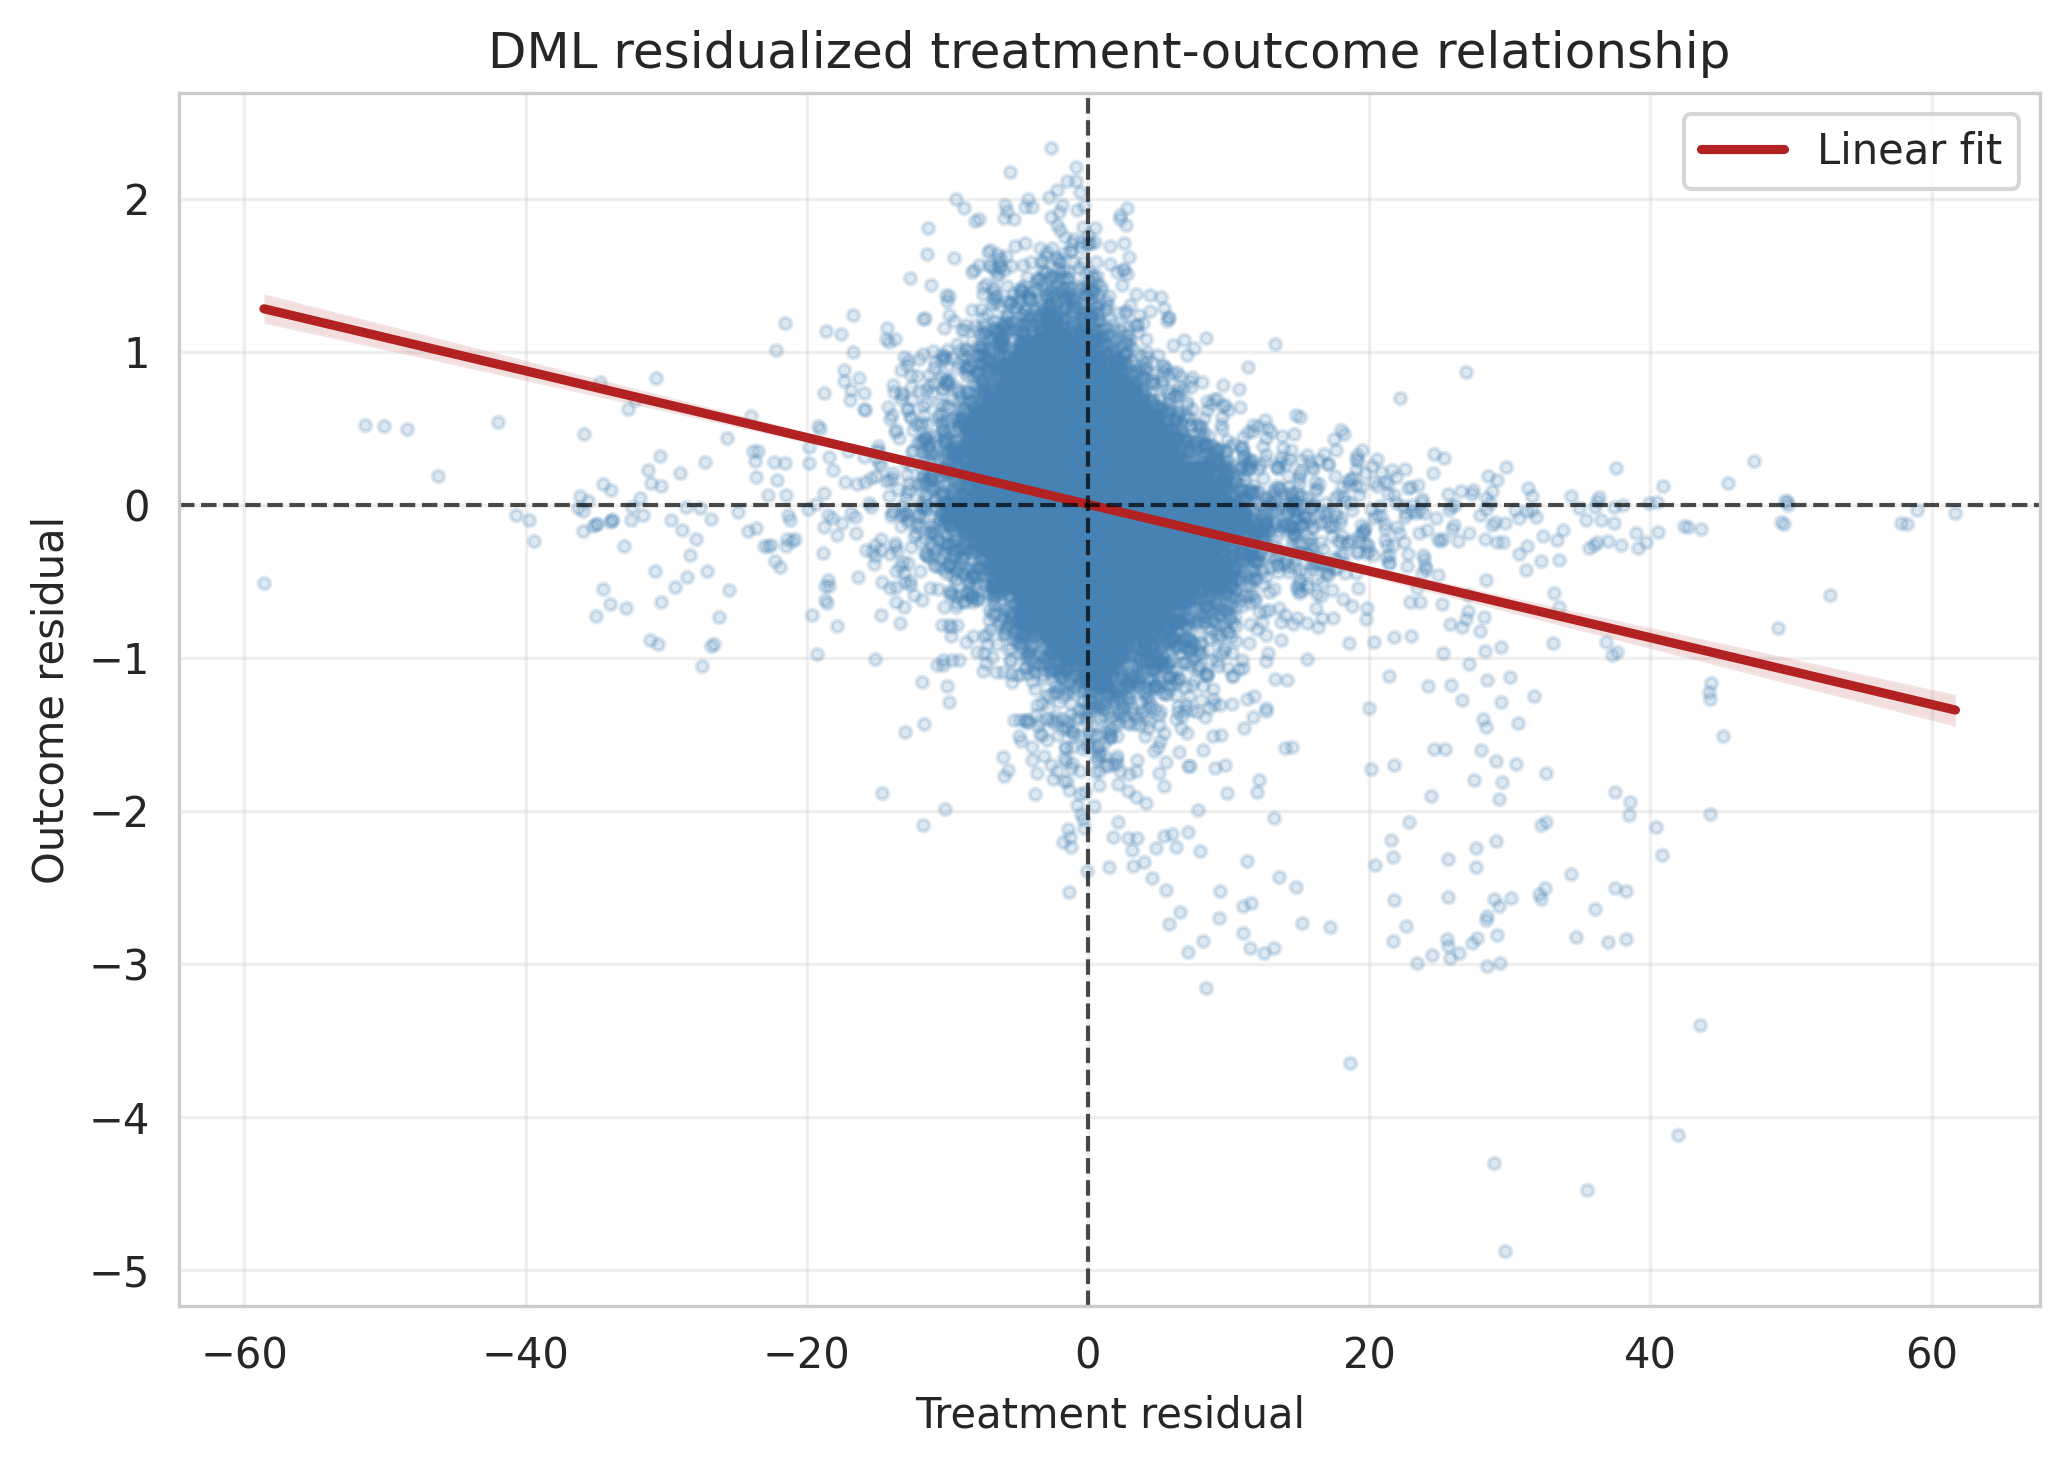
\includegraphics[width=0.78\textwidth]{Figures/dml_residualized_treatment_outcome_linear.png}}{\fbox{\parbox{0.78\textwidth}{\centering Add \texttt{dml\_residualized\_treatment\_outcome\_linear.png} to the \texttt{Figures} folder.}}}
\caption{Residualized treatment-outcome relationship after controlling for pre-pricing covariates with Double Machine Learning. The negative fitted slope is consistent with the expected demand response to higher prices.}
\label{fig:dml-residualized-linear}
\end{figure}

\begin{figure}[htbp]
\centering
\IfFileExists{Figures/cate_sales_spec_grid.png}{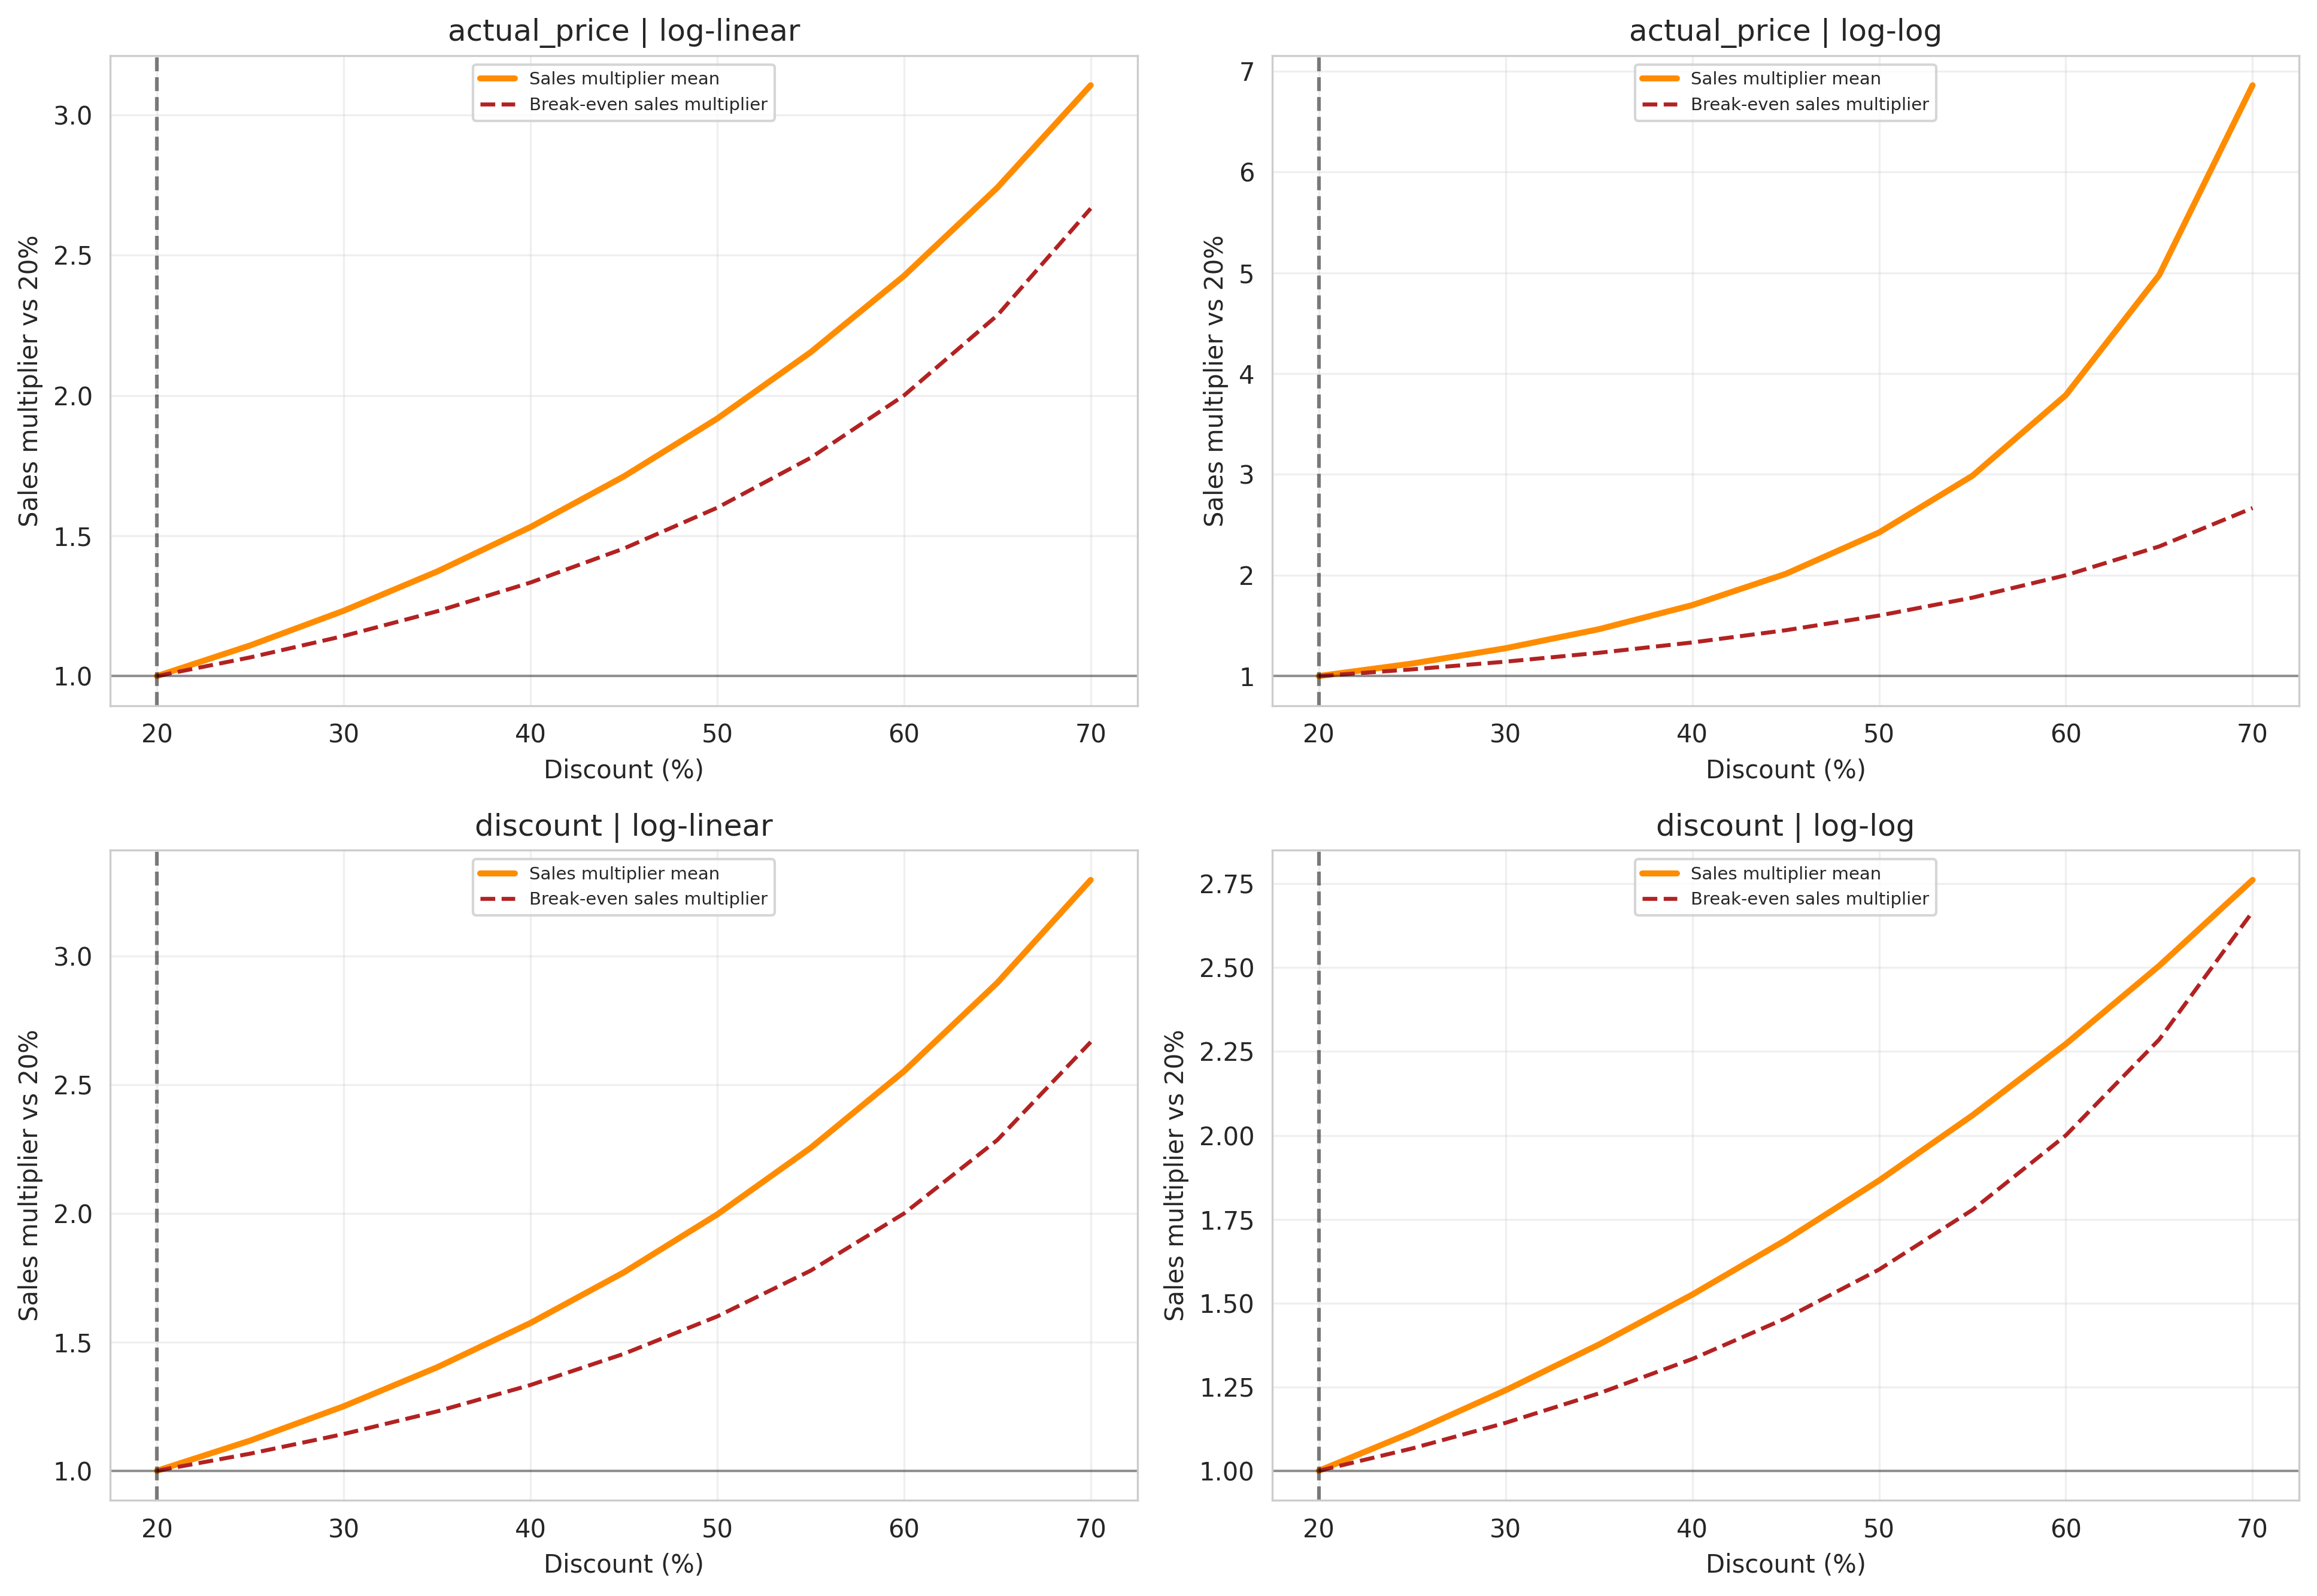
\includegraphics[width=0.95\textwidth]{Figures/cate_sales_spec_grid.png}}{\fbox{\parbox{0.95\textwidth}{\centering Add \texttt{cate\_sales\_spec\_grid.png} to the \texttt{Figures} folder.}}}
\caption{CATE-based comparison of treatment encoding and functional form. The log-linear specification using discounted price produces smoother and more economically reasonable sales-response curves than log-log or discount-based alternatives.}
\label{fig:cate-sales-spec-grid}
\end{figure}

Figure~\ref{fig:cate-sales-spec-grid} provides the empirical counterpart to the specification argument. The log-log specifications produce more polarized curves, while the log-linear specifications generate smoother responses with more plausible interior optima. Among the log-linear alternatives, the discounted-price specification is preferred because it is aligned with the revenue objective and because the treatment nuisance model is substantially stronger than in the discount-based specifications. The selected specification therefore combines a suitable revenue geometry with a stronger treatment nuisance model and smoother simulated response curves.

\section{CATE Estimation with Causal Forest}
\label{sec:cate-estimation}

A global $\hat{\beta}$ is useful for comparing specifications, but the optimizer needs one price-response curve per reference-week. To obtain heterogeneous effects, the residualized training data from the DML step are passed to EconML's \texttt{CausalForest}. The forest is fitted with $\tilde{Y}$ as the target, $\tilde{T}$ as the treatment, and the pre-pricing covariates $X$ as heterogeneity features.

The nuisance models are fitted outside the forest using the LightGBM residualization described in Section~\ref{sec:specification-dml}. The forest is therefore used only as the heterogeneous final stage, estimating how the residualized price effect varies across reference-weeks. Its configuration is reported in Appendix~\ref{AppendixA}.

Following the transformation introduced in Section~\ref{sec:local-effects-markdown-curves}, each local semi-elasticity is converted into a markdown curve over the operational discount grid from 20\% to 70\%, normalized at the 20\% reference discount. These reference-week-level sales multiplier curves are the causal input passed to the optimizer.

The estimated local effects are summarized in Chapter~\ref{Chapter5}, together with the global curve comparison and reference-level examples.
\chapter{Results}

\label{Chapter5}

\section{Final Model and Predictive Performance}

The final model is the log-linear DML specification using discounted price as the treatment, with a Causal Forest final stage to estimate heterogeneous price effects at reference-week level. As justified in Section~\ref{sec:specification-dml}, this choice aligns the demand specification with the revenue objective and allows interior revenue optima.

The outcome is season-normalized weekly units sold, used in logarithmic scale, so the estimated effects are local semi-elasticities. The first diagnostic compares predictive performance against the existing LightGBM baseline. Prediction accuracy is not the main objective, but it remains relevant because the resulting elasticity curves must remain compatible with the existing optimization module.

\begin{table}[h]
\centering
\small
\begin{tabular}{llrrr}
\toprule
\textbf{Model} & \textbf{Split} & \textbf{WMAPE} & \textbf{$R^2$} & \textbf{N} \\
\midrule
LightGBM baseline & Train OOF & 0.312 & 0.797 & 33,691 \\
LightGBM baseline & Test & 0.425 & 0.706 & 12,136 \\
Causal Forest & Train OOF & 0.305 & 0.815 & 33,691 \\
Causal Forest & Test observed sales & 0.417 & 0.731 & 12,136 \\
\bottomrule
\end{tabular}
\caption{Predictive performance of the LightGBM baseline and final Causal Forest model. Test metrics are computed on the 12,136 held-out reference-week rows with observed sales.}
\label{tab:model-predictive-performance}
\end{table}

Table~\ref{tab:model-predictive-performance} shows that the causal specification does not reduce predictive quality. On the observed holdout rows, the Causal Forest obtains a slightly lower WMAPE and a slightly higher $R^2$ than the LightGBM baseline. However, predictive metrics are not enough in this application: the model must also generate plausible counterfactual demand curves when alternative discounts are simulated.

\section{Economic Quality of the Elasticity Curves}

The main evaluation criterion is whether the generated elasticity curves are economically reasonable and useful for the markdown optimizer. In the existing predictive approach, simulated curves often lead to boundary recommendations, where the optimizer recommends the minimum allowed discount instead of finding a balanced middle ground. This is problematic because markdown pricing should involve a trade-off between volume and unit price.

The LightGBM baseline and the final Causal Forest model are compared using curve-quality diagnostics: the share of recommendations at the minimum limit, the share at the maximum limit, the share of interior optima, the median optimal discount, and the share of curves that cross the break-even sales multiplier.

\begin{table}[h]
\centering
\small
\begin{tabular}{lrrrrr}
\toprule
\textbf{Model} & \textbf{Min limit} & \textbf{Max limit} & \textbf{Interior} & \textbf{Median opt.} & \textbf{Break-even} \\
\midrule
LightGBM baseline & 75.8\% & 4.4\% & 19.8\% & 20\% & 24.2\% \\
Causal Forest & 37.7\% & 7.6\% & 54.7\% & 35\% & 62.3\% \\
\bottomrule
\end{tabular}
\caption{Curve-quality diagnostics over the operational discount grid. The diagnostics emphasize robust shares rather than unstable mean revenue multipliers.}
\label{tab:curve-quality}
\end{table}

Table~\ref{tab:curve-quality} shows a clear improvement in curve quality. The LightGBM baseline places 75.8\% of optimal recommendations at the minimum allowed discount, confirming this tendency to get stuck at the lowest boundary. By contrast, the Causal Forest reduces minimum-limit optima to 37.7\% and increases interior optima to 54.7\%.

This improvement is consistent with the specification analysis in Section~\ref{sec:specification-dml}. The selected log-linear form can produce interior revenue optima, and the causal model generates curves that better reflect the markdown trade-off: deeper discounts increase demand, but the additional volume does not always compensate for the lower price.

\begin{figure}[h]
\centering
\IfFileExists{Figures/global_comparison.png}{
\includegraphics[width=0.9\textwidth]{global_comparison}}{\fbox{\parbox{0.9\textwidth}{\centering Add \texttt{global\_comparison.png} to the \texttt{Figures} folder.}}}
\caption{Aggregate sales multiplier curves for the LightGBM baseline and the final Causal Forest model. Sales are normalized at the 20\% reference discount. The break-even line represents the sales increase required to compensate for the lower unit price.}
\label{fig:global-comparison}
\end{figure}

Figure~\ref{fig:global-comparison} supports the same conclusion. The Causal Forest curve shows a smoother and more economically meaningful demand response than the predictive baseline. As discounts increase, the causal model predicts higher sales multipliers, but not enough to make the deepest discount always optimal.

Because revenue multiplier averages can be unstable when predicted demand at the reference discount is very small, the analysis emphasizes robust curve-quality measures such as interior optima and break-even crossings.

\section{Heterogeneous Treatment Effects}

The final model estimates a different local price effect for each reference-week. This is necessary because the optimizer operates at reference-week level, not only at aggregate level. A single average price effect would ignore differences across product families, stock positions, price levels, and moments of the sales campaign.

The distribution of estimated CATE values is economically reasonable. The estimated local effects are negative across the holdout sample, meaning that higher prices are associated with lower expected demand after controlling for pre-pricing confounders.

\begin{table}[h]
\centering
\small
\begin{tabular}{lr}
\toprule
\textbf{Statistic} & \textbf{$\hat{\tau}$} \\
\midrule
Mean & -0.031 \\
Median & -0.024 \\
Standard deviation & 0.027 \\
P5 & -0.087 \\
P25 & -0.044 \\
P75 & -0.008 \\
P95 & -0.001 \\
Share negative & 100\% \\
\bottomrule
\end{tabular}
\caption{Distribution of Causal Forest local semi-elasticities on the holdout sample. Negative values indicate that higher prices reduce expected demand.}
\label{tab:cate-distribution}
\end{table}

The mean local semi-elasticity is approximately -0.031, which means that, on average, a one-euro increase in price reduces normalized weekly demand by approximately 3.1\%, holding the observed pre-pricing context fixed. The median effect is slightly smaller in magnitude, around 2.4\%, while the 5th and 95th percentiles show clear heterogeneity across reference-weeks.

This spread confirms that the model is not applying the same demand response to every product. Some reference-weeks are more price-sensitive than others, consistent with differences in product type, price level, stock pressure, sales momentum, and timing within the sales period.

\IfFileExists{Figures/cate_heterogeneity.pdf}{%
\begin{figure}[h]
\centering
\includegraphics[width=0.9\textwidth]{cate_heterogeneity}
\caption{Distribution of estimated local price effects. Negative values indicate that higher prices reduce expected demand. The spread of the distribution shows that the final model captures heterogeneous markdown sensitivity across reference-weeks.}
\label{fig:cate-heterogeneity}
\end{figure}
}{}

\section{Reference-Level Examples}

The previous sections evaluate the model at aggregate level, but the practical use case requires one elasticity curve per reference-week. Figure~\ref{fig:reference-examples} compares the LightGBM baseline and the Causal Forest curves for selected product examples.

\begin{figure}[h]
\centering
\IfFileExists{Figures/elasticity_examples_baseline_vs_causal.png}{
\includegraphics[width=0.95\textwidth]{elasticity_examples_baseline_vs_causal}}{\fbox{\parbox{0.95\textwidth}{\centering Add \texttt{elasticity\_examples\_baseline\_vs\_causal.png} to the \texttt{Figures} folder.}}}
\caption{Reference-level comparison between the LightGBM baseline and the Causal Forest elasticity curves for selected product examples. Sales multipliers are normalized at the 20\% reference discount and compared with the break-even multiplier.}
\label{fig:reference-examples}
\end{figure}

The examples show how the causal model changes the simulated demand response. The predictive baseline can produce flatter, irregular, or boundary-oriented curves because it is trained under the historical pricing policy. The Causal Forest curves are smoother and more aligned with the expected relationship between discounts and demand.

This matters because the existing optimization module consumes reference-week-level curves over a discount grid. The contribution of the causal model is therefore to improve the curve-generation step while keeping the optimization interface unchanged.

\section{Limitations of the Empirical Results}
\label{sec:results-limitations}

The empirical results should be interpreted within the scope of the available data and the maintained causal assumptions. First, the causal interpretation depends on unconfoundedness. Historical markdowns were not randomly assigned, and business teams may have used information that is not fully captured in the dataset. If relevant pricing drivers are missing, the estimated effects may still contain residual confounding.

Second, the curves should not be extrapolated outside the price range supported by the data. The simulations are evaluated on the operational discount grid from 20\% to 70\%, where the model has stronger empirical support.

Third, the analysis is restricted to the Spain market and the Woman division. This makes the setting more homogeneous, but limits generalization to other countries, divisions, and product groups.

Finally, the approach is static at reference-week level. It does not explicitly model stock depletion, customer anticipation, or interactions between consecutive weekly markdowns, even though markdown decisions are sequential during the sales campaign.
\chapter{Conclusion}

\label{Chapter6}

This thesis studies markdown price optimization in fashion retail from a causal machine learning perspective. The motivation comes from a practical limitation of the existing predictive pipeline: although the LightGBM baseline can forecast observed sales with reasonable accuracy, its simulated elasticity curves often lead to extreme minimum discount recommendations.

The thesis argues that this issue comes from the difference between prediction and intervention. Historical discounts are not randomly assigned; they depend on stock, previous sales, product characteristics, calendar position, and other business signals. Therefore, the observed relationship between discounts and sales does not directly represent the causal effect of changing price.

To address this problem, the thesis proposes a Double Machine Learning framework combined with a Causal Forest final stage. DML residualizes both demand and discounted price with respect to pre-pricing confounders, while the Causal Forest estimates heterogeneous local price effects at reference-week level. The final selected specification uses discounted price, the selling price after markdown, as the treatment and a log-linear outcome transformation, which is better aligned with the revenue objective and can generate interior revenue optima.

The empirical results support the usefulness of the causal approach. Predictive performance remains comparable to the LightGBM baseline, while the economic quality of the simulated markdown curves improves. The share of interior optima increases from 19.8\% to 54.7\%, the share of minimum-limit recommendations decreases from 75.8\% to 37.7\%, and the share of curves crossing the break-even line increases from 24.2\% to 62.3\%.

Overall, within the scope of the available data and the maintained identification assumptions, the proposed model produces more reasonable and actionable elasticity curves than the purely predictive baseline. Its main contribution is to improve the causal quality of the curve-generation step while remaining compatible with the existing markdown optimization framework.

%----------------------------------------------------------------------------------------
%	THESIS CONTENT - APPENDICES
%----------------------------------------------------------------------------------------

\appendix % Cue to tell LaTeX that the following "chapters" are Appendices

% Include the appendices of the thesis as separate files from the Appendices folder
% Uncomment the lines as you write the Appendices

% Appendix A

\chapter{Additional Methodological Details}

\label{AppendixA}


\section{Baseline Elasticity Simulation}

For each holdout reference-week, the predictive LightGBM baseline is evaluated over the operational discount grid from 20\% to 70\%. All contextual variables are held fixed, while the discount variable (\texttt{discount}) is changed. This creates a simulated demand curve for the same reference-week under alternative markdown decisions.

The predicted weekly sales at each discount are normalized by the prediction at the 20\% reference discount:

\begin{equation}
\text{sales multiplier}(d) =
\frac{\widehat{\text{sales}}(d)}
{\widehat{\text{sales}}(20\%)}.
\end{equation}

The break-even multiplier is the increase in units sold required to compensate for the lower discounted price:

\begin{equation}
\text{break-even}(d) =
\frac{P(20\%)}
{P(d)}
=
\frac{1-20\%}{1-d},
\end{equation}

where $P(d)$ is discounted price at discount $d$.

A simulated discount is revenue-improving relative to 20\% only when the predicted sales multiplier is above the break-even multiplier. This diagnostic is used to identify whether the predictive baseline produces economically reasonable curves or instead generates boundary-oriented recommendations.

\section{Hyperparameters}

The LightGBM nuisance models used in the DML step are trained to estimate the conditional expectation of the outcome and the treatment given the pre-pricing covariates. The same configuration is used for both nuisance models. Cross-fitting is performed using leave-one-season-out folds to reduce temporal leakage.

\begin{table}[h]
\centering
\small
\begin{tabular}{ll}
\toprule
\textbf{Hyperparameter} & \textbf{Value} \\
\midrule
Objective & regression \\
Maximum boosting iterations & 1000 \\
Learning rate & 0.01 \\
Number of leaves & 127 \\
Minimum child samples & 8 \\
Subsample fraction & 0.8 \\
Column subsample by tree & 0.8 \\
L2 regularization & 0.03 \\
Early stopping rounds & 20 \\
Random seed & 42 \\
Cross-fitting & leave-one-season-out \\
\bottomrule
\end{tabular}
\caption{Hyperparameters of the LightGBM nuisance models used in the DML residualization step.}
\label{tab:dml-hyperparams}
\end{table}

No monotonic constraint is imposed at the nuisance stage: the nuisance models estimate conditional means, while the causal price effect is captured in the final stage. Leave-one-season-out cross-fitting blocks temporal leakage and avoids predicting residuals on observations used to train the corresponding nuisance model.

The Causal Forest is used as the heterogeneous final stage after residualization. It receives the residualized outcome, the residualized treatment, and the pre-pricing covariates used as heterogeneity features.

\begin{table}[h]
\centering
\small
\begin{tabular}{ll}
\toprule
\textbf{Hyperparameter} & \textbf{Value} \\
\midrule
Number of trees & 1000 \\
Minimum samples per leaf & 80 \\
Random seed & 42 \\
Parallel jobs & -1 \\
Honest splitting & enabled \\
Inference enabled & yes \\
\bottomrule
\end{tabular}
\caption{Hyperparameters of the Causal Forest final stage.}
\label{tab:cf-hyperparams}
\end{table}

The minimum leaf size is set conservatively to reduce noisy reference-level treatment effects. This is important because the final output is not only used for average interpretation, but also for individual reference-week elasticity curves. The nuisance models are not internal to the forest; they are fitted separately with LightGBM and their residuals are passed to \texttt{CausalForest}.

% Appendix B

\chapter{Source Code}

\label{AppendixB}

The source code associated with this thesis is available in the project GitHub repository:

\begin{center}
\url{https://github.com/jowelhub/master-thesis-causal-machine-learning}
\end{center}

Because this project was developed in collaboration with Mango, the original datasets cannot be made public. For this reason, the repository does not include the internal CSV files used in the empirical analysis. Instead, it contains a clean thesis-oriented notebook that documents the modelling workflow and preserves the outputs needed to understand the implementation. The notebook is intended to show the main steps of the analysis, including data preparation logic, baseline modelling, Double Machine Learning residualization, Causal Forest estimation, markdown-curve simulation, and diagnostic plots.

During the research process, several exploratory notebooks were developed internally to test alternative specifications, debug the modelling pipeline, and compare different modelling choices. These intermediate notebooks are not included in the public repository, because they were part of the internal research workflow and depend on private data sources. The public notebook is therefore a curated version prepared specifically for the thesis submission and presentation: it focuses on the final methodology and results rather than on every exploratory iteration.

In parallel, an internal production-oriented implementation of the causal machine learning framework was developed within Mango's private codebase. This implementation organizes the workflow using Python classes and is designed to run operational tasks through Apache Airflow DAGs on Databricks clusters. That internal implementation contains company-specific infrastructure, data access logic, and deployment details, so it cannot be shared publicly. The public GitHub repository should therefore be understood as the reproducible thesis-facing version of the work, while the private Mango repository contains the internal engineering implementation.
%\include{Appendices/AppendixC}

%----------------------------------------------------------------------------------------
%	BIBLIOGRAPHY
%----------------------------------------------------------------------------------------

\printbibliography[heading=bibintoc]

%----------------------------------------------------------------------------------------

\end{document}  
